\documentclass{article}[11pt]


%\documentclass[runningheads,a4paper]{llncs}
%\usepackage{hyperref}
%\usepackage{ amssymb }


%\gasset{frame=false} % switch to true to add frames
%\parindent=0pt

%\usepackage{bussproofs}
%\usepackage{varwidth}
%\usepackage{xspace}
%\usepackage{verbatim}


\usepackage[lmargin=4cm, rmargin=4cm, tmargin=3cm, bmargin=3cm]{geometry}
\usepackage{algpseudocode}


\usepackage{url}
\usepackage{multirow} 
\usepackage{mathtools}
\usepackage{stmaryrd}
\DeclarePairedDelimiter{\ceil}{\lceil}{\rceil}
\DeclarePairedDelimiter{\floor}{\lfloor}{\rfloor} 
%\usepackage{xspace}
\usepackage{latexsym,amsmath,amsfonts,amssymb,stmaryrd}
\let\proof\relax
\let\endproof\relax 
\usepackage{amsthm} 
\usepackage{tikz}
\usepackage{tikz-qtree}
\usepackage{tikz-qtree-compat}

\usepackage{listings}
\usepackage{chngpage}
\DeclareMathAlphabet{\mathpzc}{OT1}{pzc}{m}{it}

\usepackage{ amssymb }
\usepackage{soul}

\usepackage{tipa}
\usepackage{stmaryrd}

\usepackage{verbatim} 
\usepackage{epsfig} 
\usepackage{graphics}
\usepackage{ mathrsfs }
\usepackage{hyperref}
\usepackage{multicol}

\usepackage{epigraph}


% \usepackage{tipa}
\usepackage{graphicx}   
%\usepackage{url}
\usepackage{wrapfig}  
\usepackage{bm}   
\usepackage{epstopdf}  
\usepackage{ upgreek }
\usepackage[all,cmtip]{xy}
 
% \usepackage{float} 
% \usepackage[lofdepth,lotdepth]{subfig}
%\usepackage{graphicx}
\usepackage[T1]{fontenc} 
\usepackage[utf8]{inputenc}
\usepackage{etoolbox}
\usepackage{textcomp}

\usepackage{mdwtab}
\usepackage{syntax} 

\renewcommand{\syntleft}{}          % do not display '<' associated with variable, for example <A>
\renewcommand{\syntright}{}         % do not display '>' associated with variable, for example <A>


\makeatletter 
\patchcmd{\maketitle}{\@copyrightspace}{}{}{}
\makeatother 
\usepackage{mathpartir}
%\usepackage{enumitem}

%\usepackage{supertabular} 
%\usepackage{soul}
\usepackage[all]{xy}
\usepackage{xifthen}
\usepackage{placeins} 
\usepackage{amsthm}
\usepackage{amsmath}


\usepackage{pgf}
\usepackage{tikz}
\usetikzlibrary{arrows,automata}
\tikzset{initial text={}}
\usetikzlibrary{calc,shapes.multipart,chains,arrows}
%prevents second paragraph indentations 
%\usepackage{parskip}
% \usepackage{floatrow}
\usepackage{tabularx} % in the preamble
\usepackage{bm}
\usepackage{caption}
\usepackage{subcaption} 

%\input{mac}

\newtheorem{theorem}{Theorem}
\newtheorem{lemma}[theorem]{Lemma}





\newenvironment{mathprooftree}
  {\varwidth{.9\textwidth}\centering\leavevmode}
  {\DisplayProof\endvarwidth}


\newcommand{\qm}{\overline{Q}\overline{m}}

\newcommand{\myparagraph}[1]{\paragraph{#1}\mbox{}\\}
\newcommand\myeq{\stackrel{\mathclap{\normalfont\mbox{\scriptsize{def}}}}{=}}

\title{Bases formelles du TAL  \\ DM sur les $\epsilon$-transitions }

\author{Pierre-Léo Bégay}
\date{À me rendre le 6 mars 2020}
\theoremstyle{definition}
\newtheorem{exmp}{Exemple}
   

\begin{document}
 
\maketitle
\pagestyle{empty} %
\thispagestyle{empty}

\newpage
%% Attention: pas plus d'un recto-verso!
% Ne conservez pas les questions

\section{$\epsilon$-transitions}

\subsection{Définitions}

On donne parfois la définition suivante d'un AFND : 


\[
A =  \big \langle Q,\Sigma,q_0,F,\delta \big \rangle
\]

\begin{itemize}
\item[] $Q$ ensemble fini d'états
\item[] $\Sigma$ l'alphabet (ensemble de lettres)
\item[] $q_0$ l'état initial
\item[] $F \subseteq Q$, les états terminaux
\item[] $\delta$ fonction de $(Q \times (\Sigma \cup \{\epsilon\}))$ dans $2^Q$ 
\end{itemize}

Par rapport à la définition du cours, on revient à un seul état initial et qu'on permet d'étiqueter des transitions par $\epsilon$. Ces transitions, appelées $\epsilon$-transitions, sont \textit{gratuites}, par contraste avec les transitions normales qui \textit{consomment} une lettre chaque fois qu'on les emprunte. La notion d'acceptation est sinon la même que pour les AFND qu'on a déjà vus. 

\subsection{Exemples}



\begin{figure}[!h]
\centering

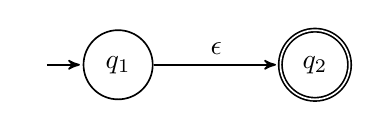
\begin{tikzpicture}[->,>=stealth',shorten >=1pt,auto,node distance=2.5cm,
                    semithick]
  \tikzstyle{every state}=[fill=white,text=black]
  \tikzstyle{place}=[rectangle,draw=black,fill=white, minimum size=7mm]


  \node[initial, state] (S)                    {$q_1$};
  \node[state,accepting] (A)      [right of=S]                {$q_2$};

  \path (S) edge      []        node {$\epsilon$} (A);
\end{tikzpicture}
\caption{Automate $A_1$}
\end{figure}

Dans l'automate $A_1$, aucune transition par lettre n'est possible, ce qui empêche d'accepter tout mot autre que le mot vide. Ce dernier est cependant reconnu car on peut emprunter \textit{gratuitement} l'unique transition et atterrir dans un état terminal.


\begin{figure}[!h]
\centering

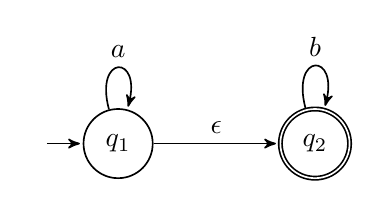
\begin{tikzpicture}[->,>=stealth',shorten >=1pt,auto,node distance=2.5cm,
                    semithick]
  \tikzstyle{every state}=[fill=white,text=black]
  \tikzstyle{place}=[rectangle,draw=black,fill=white, minimum size=7mm]


  \node[initial, state] (S)                    {$q_1$};
  \node[state,accepting] (A)      [right of=S]                {$q_2$};

  \path (S) edge[loop above]              node {$a$} (S)
(S) edge      []        node {$\epsilon$} (A)
 (A) edge[loop above]              node {$b$} (A);
\end{tikzpicture}
\caption{Automate $A_2$}
\end{figure}
\newpage
L'automate $A_2$ reconnait quant à lui le langage $a^*b^*$. En effet, on peut boucler avec des $a$ sur $q_1$ puis, une fois qu'on a fini, on passe gratuitement à $q_2$ (sans consommer de $a$ ou de $b$) où on peut boucler avec des $b$ jusqu'à avoir fini le mot.

\begin{figure}[!ht]
\centering

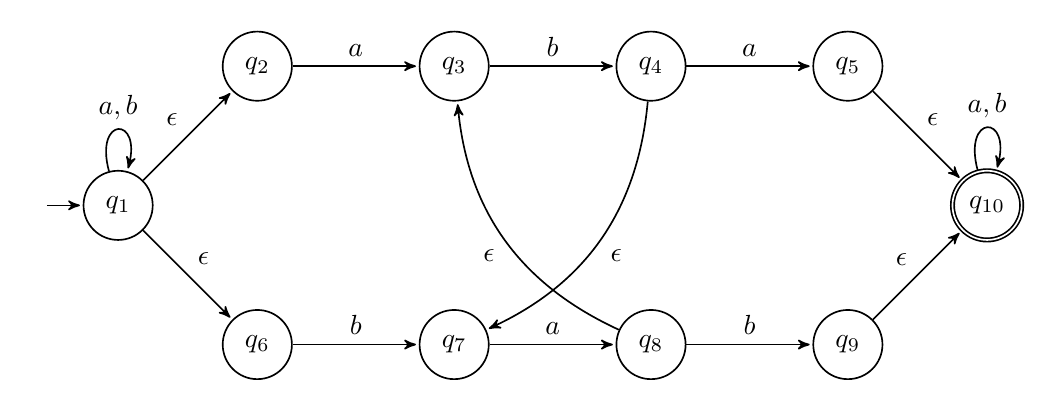
\begin{tikzpicture}[->,>=stealth',shorten >=1pt,auto,node distance=2.5cm,
                    semithick]
  \tikzstyle{every state}=[fill=white,text=black]
  \tikzstyle{place}=[rectangle,draw=black,fill=white, minimum size=7mm]


  \node[initial, state] (S)                    {$q_1$};
  \node[state] (A)      [above right of=S]                {$q_2$};
  \node[state] (B)      [right of=A]                {$q_3$};
  \node[state] (C)      [right of=B]                {$q_4$};
    \node[state] (D)      [right of=C]                {$q_5$};
  \node[state] (E)      [below right of=S]                {$q_6$};
  \node[state] (F)      [right of=E]                {$q_7$};
    \node[state] (G)      [right of=F]                {$q_8$};    \node[state] (H)      [right of=G]                {$q_9$};
        \node[state,accepting] (I)      [above right of=H]                {$q_{10}$};
  
  \path (S) edge[loop above]              node {$a,b$} (S)
 (I) edge[loop above]              node {$a,b$} (I)
(S) edge      []        node {$\epsilon$} (A)
(A) edge      []        node {$a$} (B)
(B) edge      []        node {$b$} (C)
(C) edge      []        node {$a$} (D)
(D) edge      []        node {$\epsilon$} (I)
(S) edge      []        node {$\epsilon$} (E)
(E) edge      []        node {$b$} (F)
(F) edge      []        node {$a$} (G)
(G) edge      []        node {$b$} (H)
(H) edge      []        node {$\epsilon$} (I)
(C) edge      [bend left]        node {$\epsilon$} (F)
(G) edge      [bend left]        node {$\epsilon$} (B);
\end{tikzpicture}
\caption{Automate $A_3$}
\end{figure}

Enfin, l'automate $A_3$, proche d'un qu'on a vu en cours, reconnaît quant à lui le langage $\Sigma^*aba\Sigma^* + \Sigma^*bab\Sigma^*$ (les deux $\epsilon$-transitions en croix ne permettent pas d'accepter plus de mots).



\section{Lecture d'automates avec $\epsilon$-transitions}


Décrivez les langages reconnus par les automates $A_4$, $A_5$ et $A_6$ à l'aide d'une expression rationelle. Essayez de justifier, au moins informellement, votre réponse. 

\begin{figure}[!h]
\centering

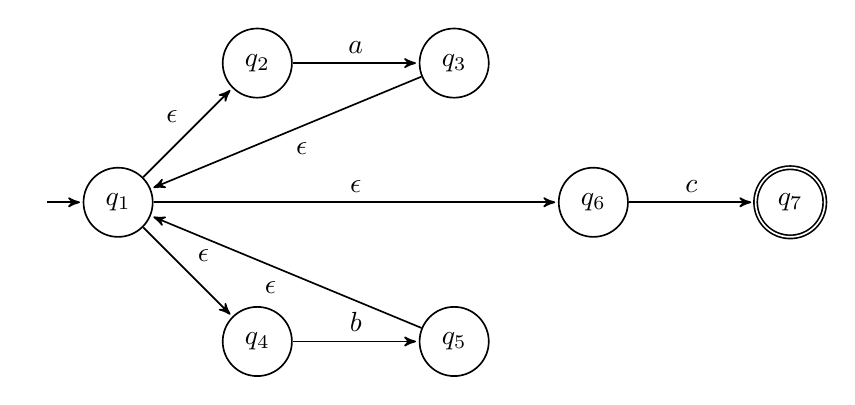
\begin{tikzpicture}[->,>=stealth',shorten >=1pt,auto,node distance=2.5cm,
                    semithick]
  \tikzstyle{every state}=[fill=white,text=black]
  \tikzstyle{place}=[rectangle,draw=black,fill=white, minimum size=7mm]


  \node[initial, state] (S)                    {$q_1$};
  \node[state] (A)      [above right of=S]                {$q_2$};
  \node[state] (B)      [right of=A]                {$q_3$};
  \node[state] (C)      [below right of=S]                {$q_4$};
    \node[state] (D)      [right of=C]                {$q_5$};
  \node[state] (E)      [above right of=D]                {$q_6$};
  \node[state,accepting] (F)      [right of=E]                {$q_7$};
    
  
  \path %(I) edge[loop above]              node {$a,b$} (I)
(S) edge      []        node {$\epsilon$} (A)
(A) edge      []        node {$a$} (B)
(B) edge      []        node {$\epsilon$} (S)
(S) edge      []        node {$\epsilon$} (C)
(C) edge      []        node {$b$} (D)
(D) edge      []        node {$\epsilon$} (S)
(S) edge      []        node {$\epsilon$} (E)
(E) edge      []        node {$c$} (F);
\end{tikzpicture}
\caption{Automate $A_4$}
\end{figure}



\begin{figure}[!h]
\centering

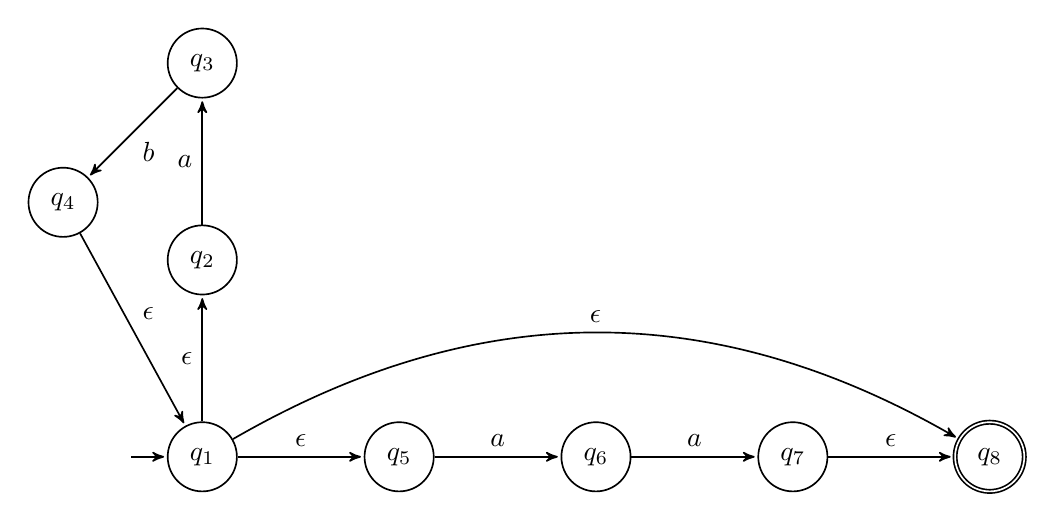
\begin{tikzpicture}[->,>=stealth',shorten >=1pt,auto,node distance=2.5cm,
                    semithick]
  \tikzstyle{every state}=[fill=white,text=black]
  \tikzstyle{place}=[rectangle,draw=black,fill=white, minimum size=7mm]


  \node[initial, state] (S)                    {$q_1$};
  \node[state] (A)      [above of=S]                {$q_2$};
  \node[state] (B)      [above of=A]                {$q_3$};
  \node[state] (C)      [below left of=B]                {$q_4$};
    \node[state] (D)      [right of=S]                {$q_5$};
  \node[state] (E)      [right of=D]                {$q_6$};
  \node[state] (F)      [right of=E]                {$q_7$};
    \node[state,accepting] (G)      [right of=F]                {$q_8$};    
    
  
  \path %(I) edge[loop above]              node {$a,b$} (I)
(S) edge      []        node {$\epsilon$} (A)
(A) edge      []        node {$a$} (B)
(B) edge      []        node {$b$} (C)
(C) edge      []        node {$\epsilon$} (S)
(S) edge      []        node {$\epsilon$} (D)
(D) edge      []        node {$a$} (E)
(E) edge      []        node {$a$} (F)
(F) edge      []        node {$\epsilon$} (G)
(S) edge      [bend left]        node {$\epsilon$} (G);
\end{tikzpicture}
\caption{Automate $A_5$}
\end{figure}

\newpage

\begin{figure}[!h]
\centering

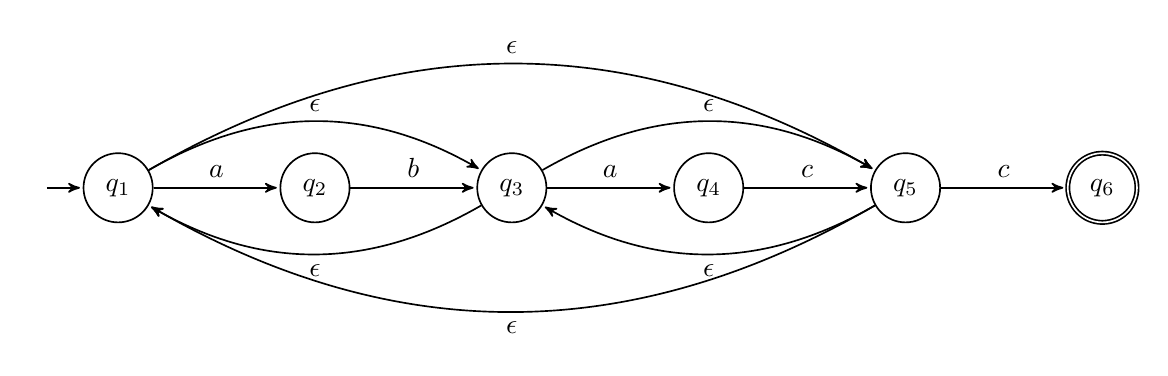
\begin{tikzpicture}[->,>=stealth',shorten >=1pt,auto,node distance=2.5cm,
                    semithick]
  \tikzstyle{every state}=[fill=white,text=black]
  \tikzstyle{place}=[rectangle,draw=black,fill=white, minimum size=7mm]


  \node[initial, state] (S)                    {$q_1$};
  \node[state] (A)      [right of=S]                {$q_2$};
  \node[state] (B)      [right of=A]                {$q_3$};
  \node[state] (C)      [right of=B]                {$q_4$};
    \node[state] (D)      [right of=C]                {$q_5$};
  \node[state,accepting] (E)      [right of=D]                {$q_6$};

    
  
  \path %(I) edge[loop above]              node {$a,b$} (I)
(S) edge      []        node {$a$} (A)
(A) edge      []        node {$b$} (B)
(S) edge      [bend left]        node {$\epsilon$} (B)
(B) edge      [bend left]        node {$\epsilon$} (S)
(B) edge      [bend left]        node {$\epsilon$} (D)
(D) edge      [bend left]        node {$\epsilon$} (B)
(S) edge      [bend left]        node {$\epsilon$} (D)
(D) edge      [bend left]        node {$\epsilon$} (S)
(B) edge      []        node {$a$} (C)
(C) edge      []        node {$c$} (D)
(D) edge      []        node {$c$} (E);
\end{tikzpicture}
\caption{Automate $A_6$}
\end{figure}

\section{Elimination d'$\epsilon$-transitions}

On propose une méthode pour éliminer les $\epsilon$-transitions s'appuyant sur la fonction $\epsilon^+$ de type $Q \rightarrow 2^Q$ définie de la façon suivante :

\begin{figure}[!h]
\begin{enumerate}
\item Si $q_j \in \delta(q_i,\epsilon)$, alors $q_j \in \epsilon^+(q_i)$
\item Si $q_j \in \epsilon^+(q_i)$ et $q_k \in \delta(q_j,\epsilon)$, alors $q_k \in \epsilon^+(q_i)$
\end{enumerate}
\caption{Définition de $\epsilon^+$}
\label{eplusdef}
\end{figure}
 
 
A partir d'un automate non-déterministe avec $\epsilon$-transitions  $\big \langle Q,\Sigma,q_0,F,\delta \big \rangle$, on génère un automate non-déterministe équivalent sans $\epsilon$-transitions  $\big \langle Q,\Sigma,q_0,F',\delta' \big \rangle$ avec l'algorithme suivant :

\begin{figure}[!h]
\begin{algorithmic}[1]
\State $F' := F$
\ForAll {$q_i \in Q$}
    \ForAll {$c \in \Sigma$}
        $\delta'(q_i,c) := \delta(q_i,c)$
    \EndFor
\EndFor
\ForAll{$q_i \in Q$ tels que $\epsilon^+(q_i) \neq \emptyset$}
	\ForAll{$q_j \in \epsilon^+(q_i)$}
		\ForAll{$c \in \Sigma$ et $q_r \in Q$ tels que $q_r \in \delta(q_j,c)$}
			\State $\delta'(q_i,c) := \delta'(q_i,c) \cup \{q_r\}$
		\EndFor
		\If {$q_j \in F$}
			\State $F' := F' \cup \{q_i\}$
		\EndIf
	\EndFor
\EndFor
\end{algorithmic}
\caption{Algorithme d'élimination des $\epsilon$-transitions}
\label{algo}
\end{figure}
\vspace{2cm}
\paragraph*{Question 1} Pour chaque automate ($A_1$ à $A_6$), calculez la fonction $\epsilon^+$ en vous servant de la définition en figure \ref{eplusdef}. Vous devriez donner l'image de chaque état, par exemple $\epsilon^+(q_1) = \{q_1,q_2\}$, $\epsilon^+(q_2) = \emptyset$ etc. 

\paragraph*{Question 2} Pour chaque automate ($A_1$ à $A_6$), appliquez l'algorithme de la figure \ref{algo}. Vous pouvez dessiner le résultat. Pas besoin de détailler tous les calculs. 

\paragraph*{Question 3} Essayez d'expliquer en français la fonction $\epsilon^+$ et l'algorithme comme si vous vouliez me convaincre qu'ils font correctement leur boulot (ce qui est le cas)\footnote{Notez que rien n'est gratuit dans l'algorithme et que chaque \textit{morceau} a un sens. Vous devriez donc tout mentionner.}. Vous pouvez vous aider d'exemples, soit tirés de la question précédente, soit originaux.

\section{Formalisation}

\paragraph*{Question 4} Donnez une formalisation de l'acceptation d'un mot dans le contexte des AFND avec $\epsilon$-transtion en adaptant la définition de $\delta^*$ donnée dans le cours.

\paragraph*{Question bonus} Les AFND avec $\epsilon$-transitions sont-ils plus ou moins expressifs\footnote{cad. permettent-ils de décrire plus ou moins de langages ?} que ceux vus en cours, où on pouvait avoir plusieurs états initiaux ?


\section{Propriétés de clôture}

\paragraph*{Question 5} Etant donnés des AFND (version $\epsilon$) représentant deux expressions rationnelles quelconques $e_1$ et $e_2$, expliquez, en vous aidant de schémas, comment construire des automates reconnaissant les expressions $e_1 + e_2$, $e_1.e_2$ et $e_1^*$.

\paragraph*{Question bonus} Répondre à la question précédente en utilisant la formalisation des automates.




\end{document} 
  


 
